\chapter{Integrating SAP Business One}
\label{chap:integrating-sap-b1}
% problem description -> for the proof of context and real life texting was neccessary to build direct connection with SAP B1
% Communication with SAP isn't straight forward and is forbidden to write into SAP tables
% the decision was that the external software will be in charge of the synchronizations (call Parcelsync directly when needed, no webhooks or calls from the Parcelsync)

In the modern landscape of daily business operations, seamless integration between external software solutions and core \ac{ERP} systems is not just a convenience; it is a necessity.
As the number of external services needed for businesses to operate grows rapidly, comes the need to integrate those with minimising tight coupling and complex (hard to maintain) dependencies.
SAP Business One, a leading \ac{ERP} solution for small to medium companies, offers robust and unimaginable capabilities, but presents unique challenges when it comes to integration with third-party software. 

This chapter dives into the complexity of establishing a direct connection with SAP Business One and its underlying database. 
Direct write interactions with database tables are highly discouraged due to potential repercussions on system warranty and technical support.
However, it is important to understand that the caution advised against direct database modifications does not arise merely from overarching restrictions, but stems from a recognition of the complex structure of SAP's database. Unauthorised alterations carry the risk of compromising the integrity of the system.
It is worth mentioning that SAP Business One's pricing model is not merely instance-based, but also user-based.
This introduces additional limitations and costs that businesses must consider and potentially accept. 
Or do they?

\section{Possible solutions}
\label{sec:possible-solutions}
% describe state of the art

Bridging the gap between SAP's robust functionalities and the needs of business utilising third-party software is not as straightforward as it might initially appear. 
In today's software environment, a common requirement is the need for a web service to programmatically transfer data between third-party applications and SAP.
Despite SAP's widespread popularity, an official solution for this specific challenge was absent for a long time.

\subsection{SAP Business One Data Interface API}
\label{subsec:sap-b1-di-api}
% low level approach with direct access to the object
% was implemented in the bachaleor's thesis however did not fullfill the expectations and was pretty much phased out in favor of the SAP Business One Service Layer

One of the foundational solutions provided by SAP is \ac{DI API}.
This low-level programming interface offers direct access to SAP Business One objects, enabling developers to perform Create, Rear, Update, Delete (\ac{CRUD}) operations on SAP data. 
The \ac{DI API} was the go-to choice for many years because it was already installed with every SAP instance and the programmer could access SAP directly via \texttt{C\#} interface already known from a SAP user interface.
However, this convenience also introduces significant limitations.
The \ac{DI API} operates through a local \textit{Component Object Model} (COM) that is installed alongside SAP Business One.
This architecture requires that any code that uses the DI API must be executed in the environment where the COM is located.
Consequently, this code must typically run on a Windows machine and is ideally written in \texttt{C\#}, which may not always align with the preferred development practices or the existing infrastructure of a company.
Despite these challenges, a workaround exists in the form of a \textit{wrapper library}.
Although this does not address the deployment environment limitations, it enables the translation of the library's existing interface into one that is compatible with other programming languages.
For example, it is then possible to port \texttt{C\#} library into Python using tools such as the \texttt{makepy} library.


\subsection{VCZ.WebService}
% Briefly present VCZ.WebService and it's drawbacks
A noteworthy solution to address several issues associated with using the \ac{DI API} alone  is the \textit{VCZ.WebService} developed by Versino, a SAP Business One supplier. 
It was one of the first web services available for SAP users operating on the \textit{SOAP} (Simple Object Access Protocol) standard. 
This makes \textit{VCZ.WebService} a good choice for data transmission between SAP and a variety of third-party software.
In particular, the connection to \textit{VCZ.WebService} uses the standard SAP user licence.

This introduces key advantages, flexibility. 
Unlike using a pure \ac{DI API}, \textit{VCZ.WebService} introduces a layer over the \ac{DI API} that allows third-party software to run in various operating systems and environments.
However, \textit{VCZ.WebService} is not without its disadvantages.
In today's world, using \ac{SOAP} is not considered a modern approach. Most programmers seek \ac{REST} services which more align with the modern architectural styles and preferences.
Since the log-in is done using a standard SAP user, a programmer using \textit{VCZ.WebService} has to use a licence provided by the company to use only for the WebService, raising security concerns.
Furthermore, at the time of writing this thesis, \textit{VCZ.WebService} is gradually being phased out in favour of newer technologies introduced in \ref{subsec:sap-b1-service-layer}.

\subsection{SAP Business One Service Layer}
\label{subsec:sap-b1-service-layer}
% Year after finishing the bachaleor's thesis, company moved to the newer version of SAP Business One (v9) which introduced SAP Business One Service Layer which finally brought simple REST-based approach for communicating with SAP with all mappings onto SAP objects and tables

The introduction of \textit{ SAP Business One Service Layer} marked an evolution in SAP integration capabilities. 
Launched with version 9 of SAP Business One, the \textit{Service Layer} is a modern \ac{REST}-based interface that handles communication with SAP systems. 
The \textit{Service Layer} is controllable only using HTTP operations, making it accessible from any programming environment able to perform HTTP requests, thus vastly broadening its applicability.

It offers a well-documented, standardised way to interact with SAP objects and perform operations similar to the ones in \ac{ERP}'s user interface. 
Featuring user-defined queries and the ability to control safe patching and posting into the SAP database.
User-defined queries are an interesting feature. They are normal SQL \texttt{SELECT} queries with the requirement to first be stored as a string in the SAP database and then called by the \textit{ Service Layer} for data retrieval.
It is very safe in this way, but fairly limiting and time-consuming for the user. 
Sadly, authentication is still done using an SAP user licence, generating a short-lived token via \textit{Service Layer} introducing a little overhead when using this service.
Both limitations will be discussed later in this chapter \ref{chap:analysis} including a possible solution.
The transition from the raw \textit{DI API} adopting \textit{SAP Business One Service Layer} reflects a broader trend towards web-based APIs for enterprise integration.
However, being a first-party solution and providing key features with seamless SAP data manipulation, it still lacks the features needed for fast data queries and it's own authentication. Business does not want to provide it's own licence for which they have to pay extra and raise a security concerns with exposing the licence.

This project proposes a new approach to overcome these challenges.
By introducing a publicly accessible solution through a reverse proxy equipped with its own authentication policies.

\section{SAP Business One Service Layer Proxy with direct Database connector}
\label{sec:sap-b1-service-layer-proxy}
% description of the SAP Business One Server Layer Proxy which was created so that company can simply integrate Parcelsync. 
Integrating SAP Business One with external applications - such as e-Commerce platforms, different warehouse solutions, and Parcelsync - presents complex challenges that existing  approaches fail to address. 
These challenges call for a new solution (or at least an enhancement of the existing one) that allows secure access to the Service Layer over the Internet without compromising SAP credentials and thus creating SAP user accounts for each user of the API.
This solution should not only allow new integration capabilities but also ensure that business can maintain the security and integrity of the SAP Business One and it's database.

\subsection{Analysis}
\label{subsec:analysis}
% analysis of the proxy
As we came to the conclusion, existing solutions for integrating SAP Business One with external applications fall short of meeting requirements of business and are not very straight forward to use in few aspects.
This analysis explores the needs for creating a proxy for SAP Business One service layer with a direct database connector.

\subsubsection{Functional requirements}
\label{subsubs:functional-requirements}
% func requirements of the proxy -> 
% - simpler authentication with basic role based access
% - proxy requests to the Service Layer
% - create database GETTER (for MS SQL DB with ODBC connector)
\begin{itemize}
    \item Implement own authentication system without compromising SAP credentials.
    \item Maintain a unified SAP login session across all user interactions.
    \item Forward requests/responses to/from the SAP Business One Service Layer.
    \item Implement a direct route to execute \texttt{SELECT} database queries bypassing the SAP Service Layer.
    \item Provide the ability to switch between production and development environments for both the SAP Service Layer and the direct database connector.
    \item Implement a simple user management system for CRUD operations on users of the Proxy.
    \item Provide authorization tools for role-based access to create admins and users.
\end{itemize}

\subsubsection{Nonfunctional requirements}
\label{subsubsec:nonfunctional-requirements}
% deployment locally to the SAP B1 instance
% CI/CD
\begin{itemize}
    \item Local deployment close to SAP Business One Instance.
    \item Continuous Integration and Continuous Deployment (\ac{CI}/\ac{CD}).
    \item Ensure that the API is accessible via the HTTPS protocol from the public network.
    \item Expose the API Proxy endpoint under a public domain name.
\end{itemize}

\subsection{Architecture}
\label{subsec:architecture}
% high level architecture of the proxy software
The architecture is designed to ensure seamless integration between external applications and SAP Business One via SAP Business One Service Layer and direct connector to the Microsoft SQL database underlying the SAP instance. 
The main part of the architecture is an application that serves as a proxy and manager of singleton connectors to the SAP Service Layer and Microsoft SQL database in both development and production environments.
This application is strategically positioned behind the \texttt{NGINX} reverse proxy which serves as the entry point for all inbound requests.

The architecture consists of following key parts:
\begin{itemize}
    \item Reverse proxy
    \item Proxy app
    \item Proxy database
    \item SAP Business One Service Layer
    \item SAP database
\end{itemize}

As illustrated in Figure \ref{img07:structurizr:landscape}, the architecture within the company network can be categorised into two principal systems. One being Proxy Server and the second SAP Business One.

\begin{figure}[p]\centering
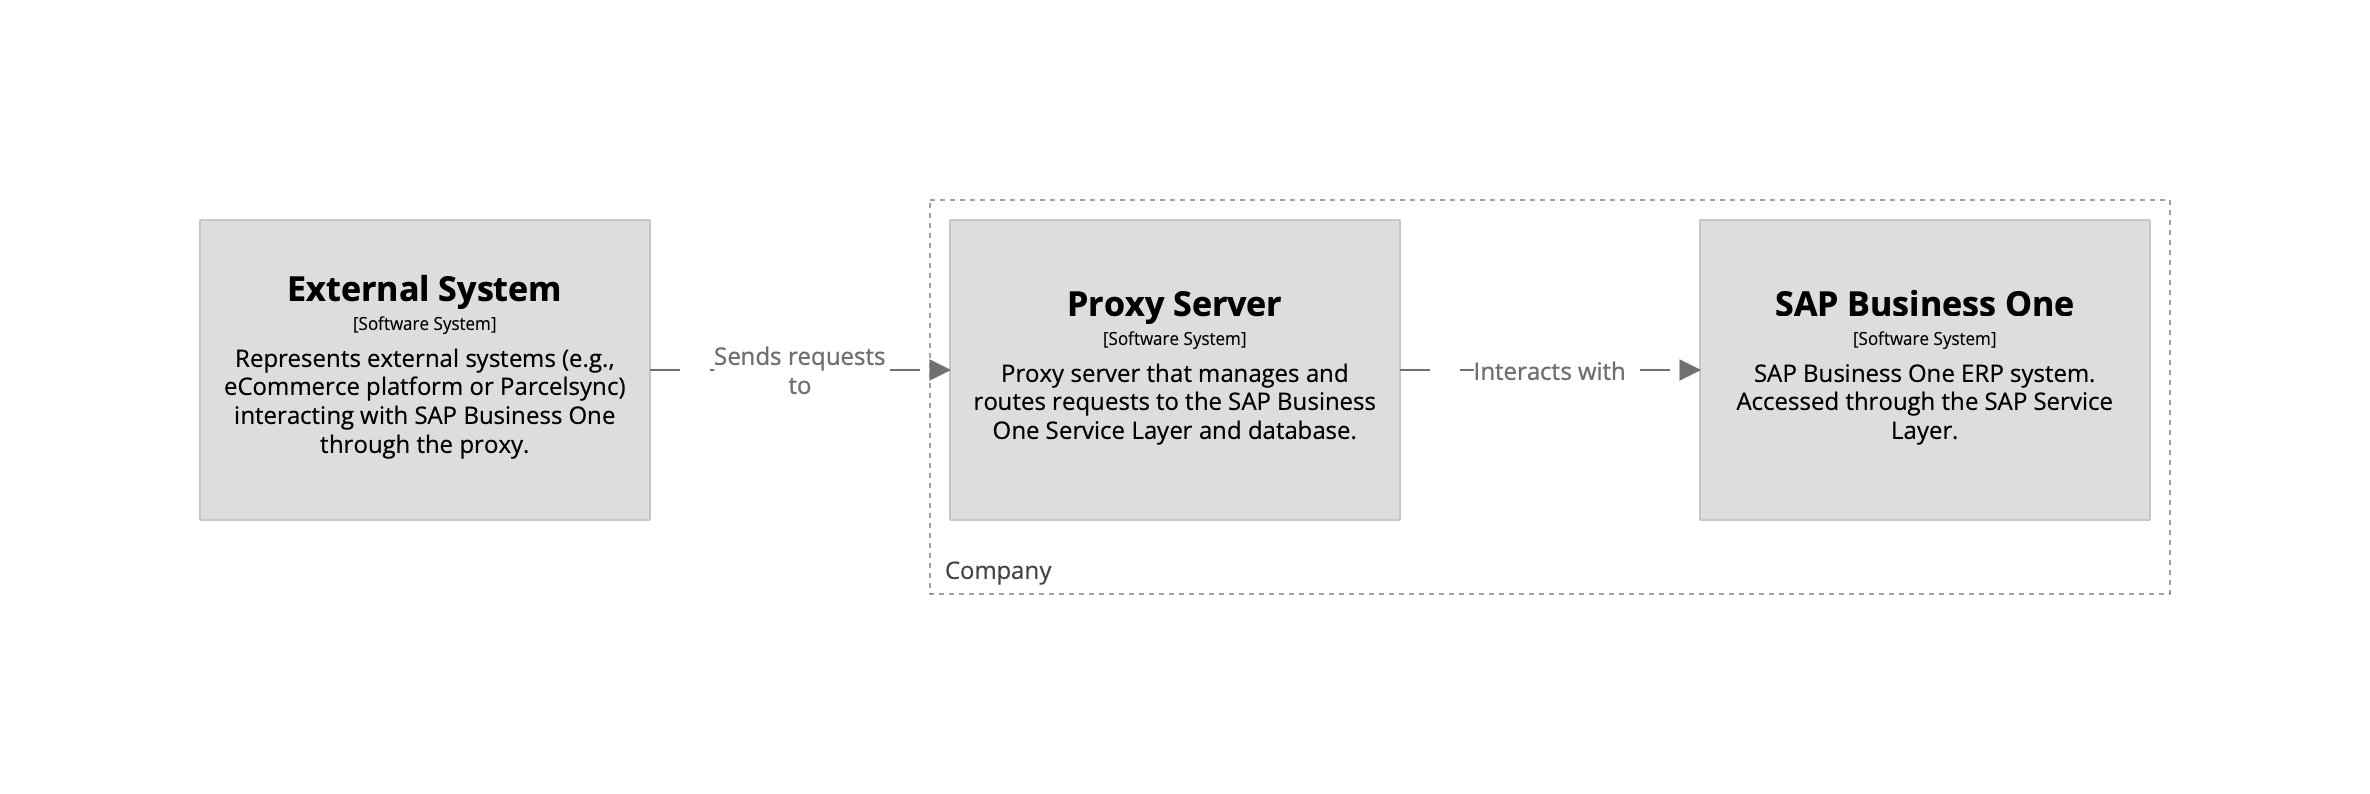
\includegraphics[width=140mm]{img/chap07/fig_structurizr-landscape.png}
\caption{C4 Landscape diagram of communication with SAP}
\label{img07:structurizr:landscape}
\end{figure}

\begin{figure}[p]\centering
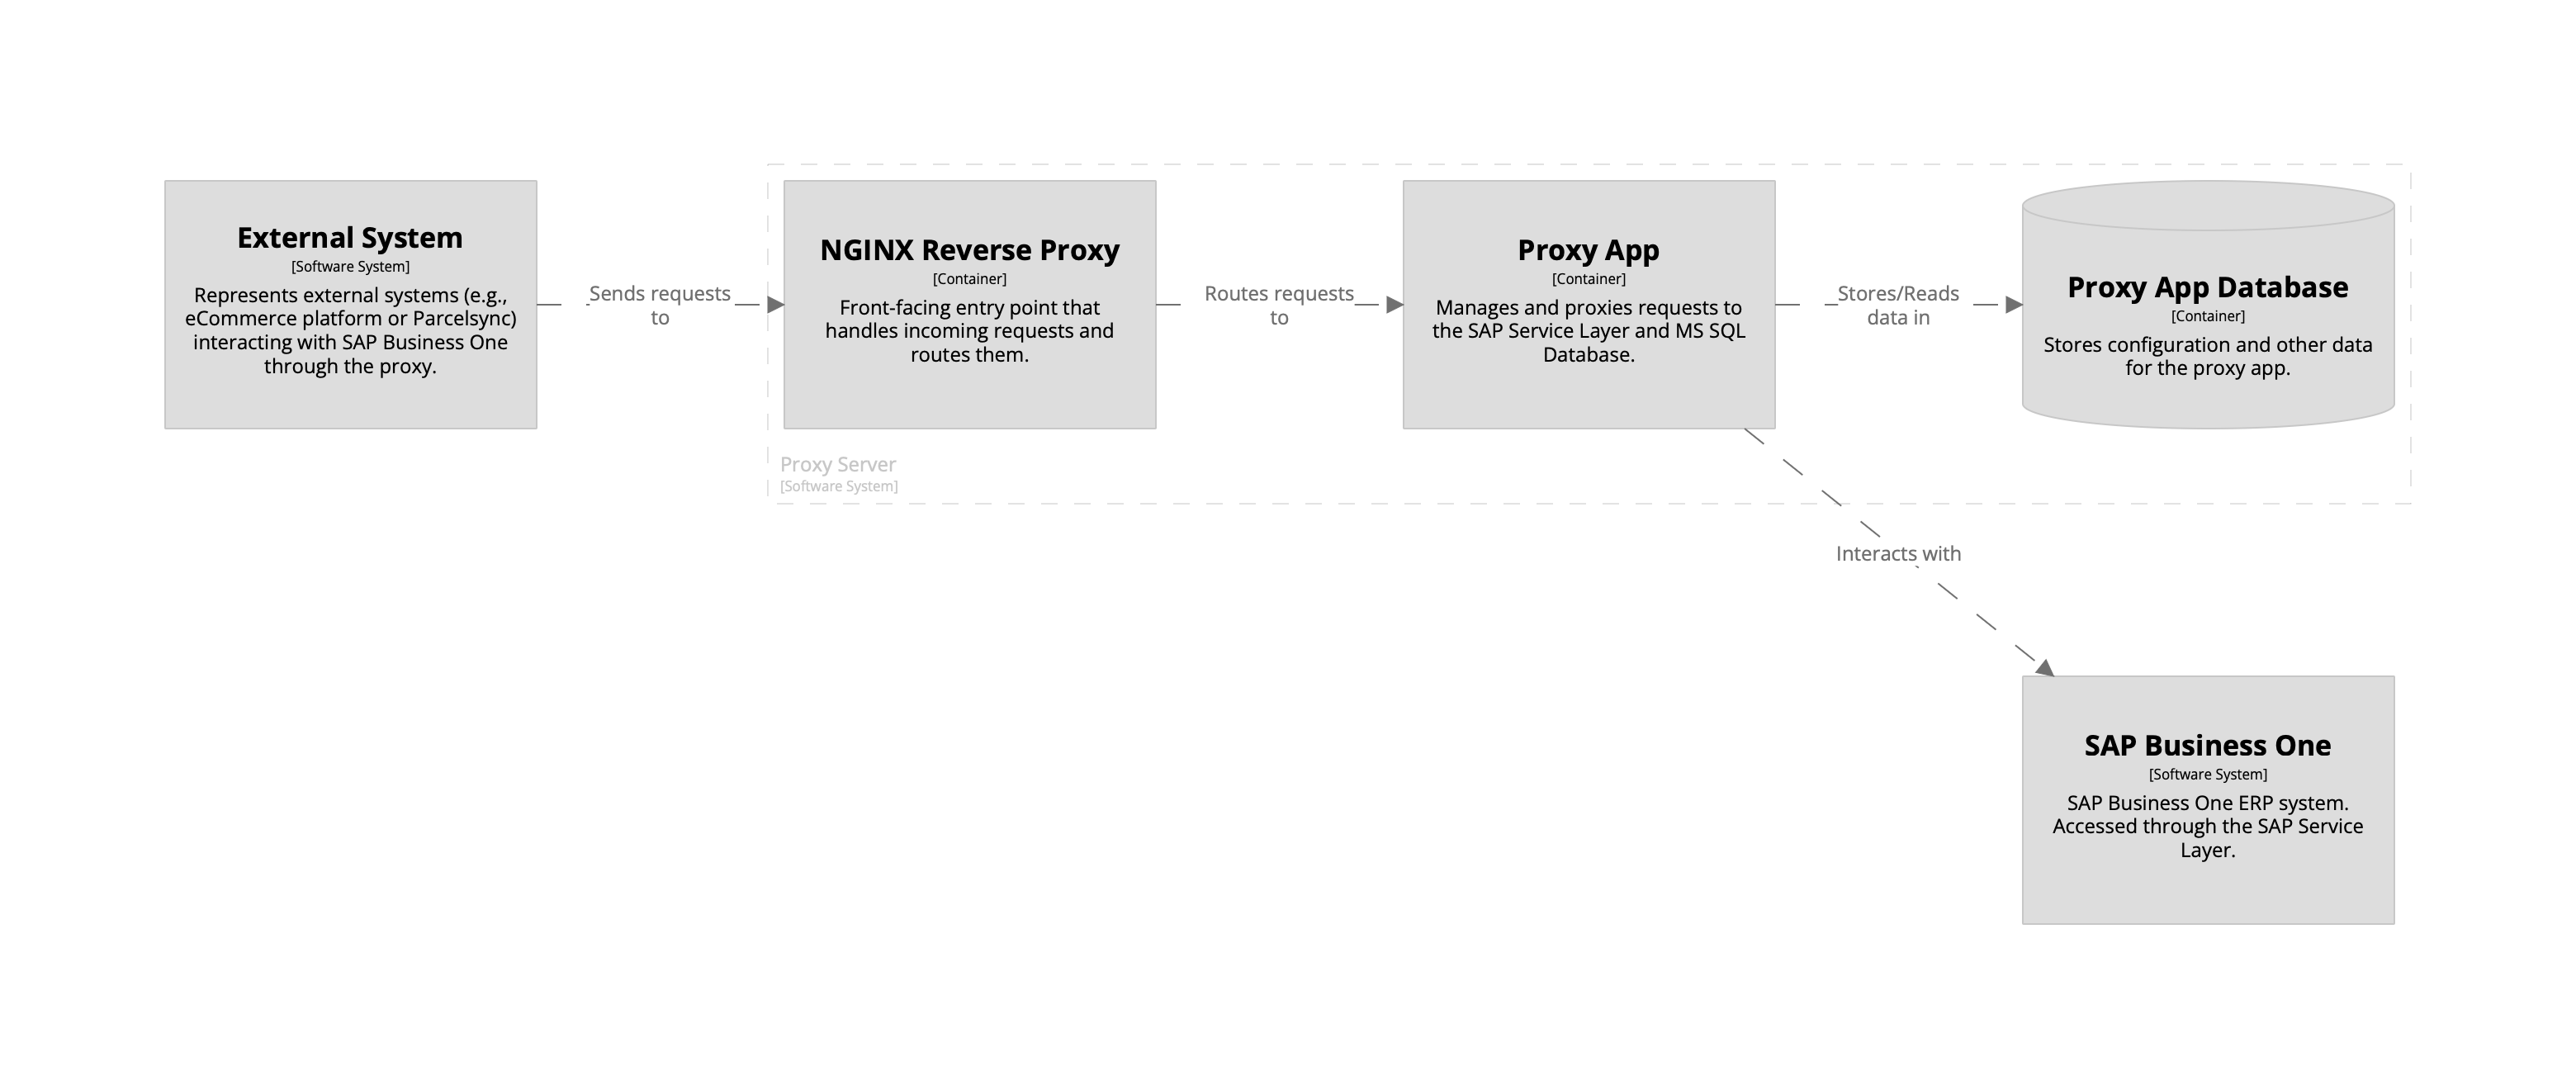
\includegraphics[width=140mm]{img/chap07/fig_structurizr-proxy-system.png}
\caption{C4 System diagram of Proxy App}
\label{img07:structurizr:system:proxy}
\end{figure}

\begin{figure}[p]\centering
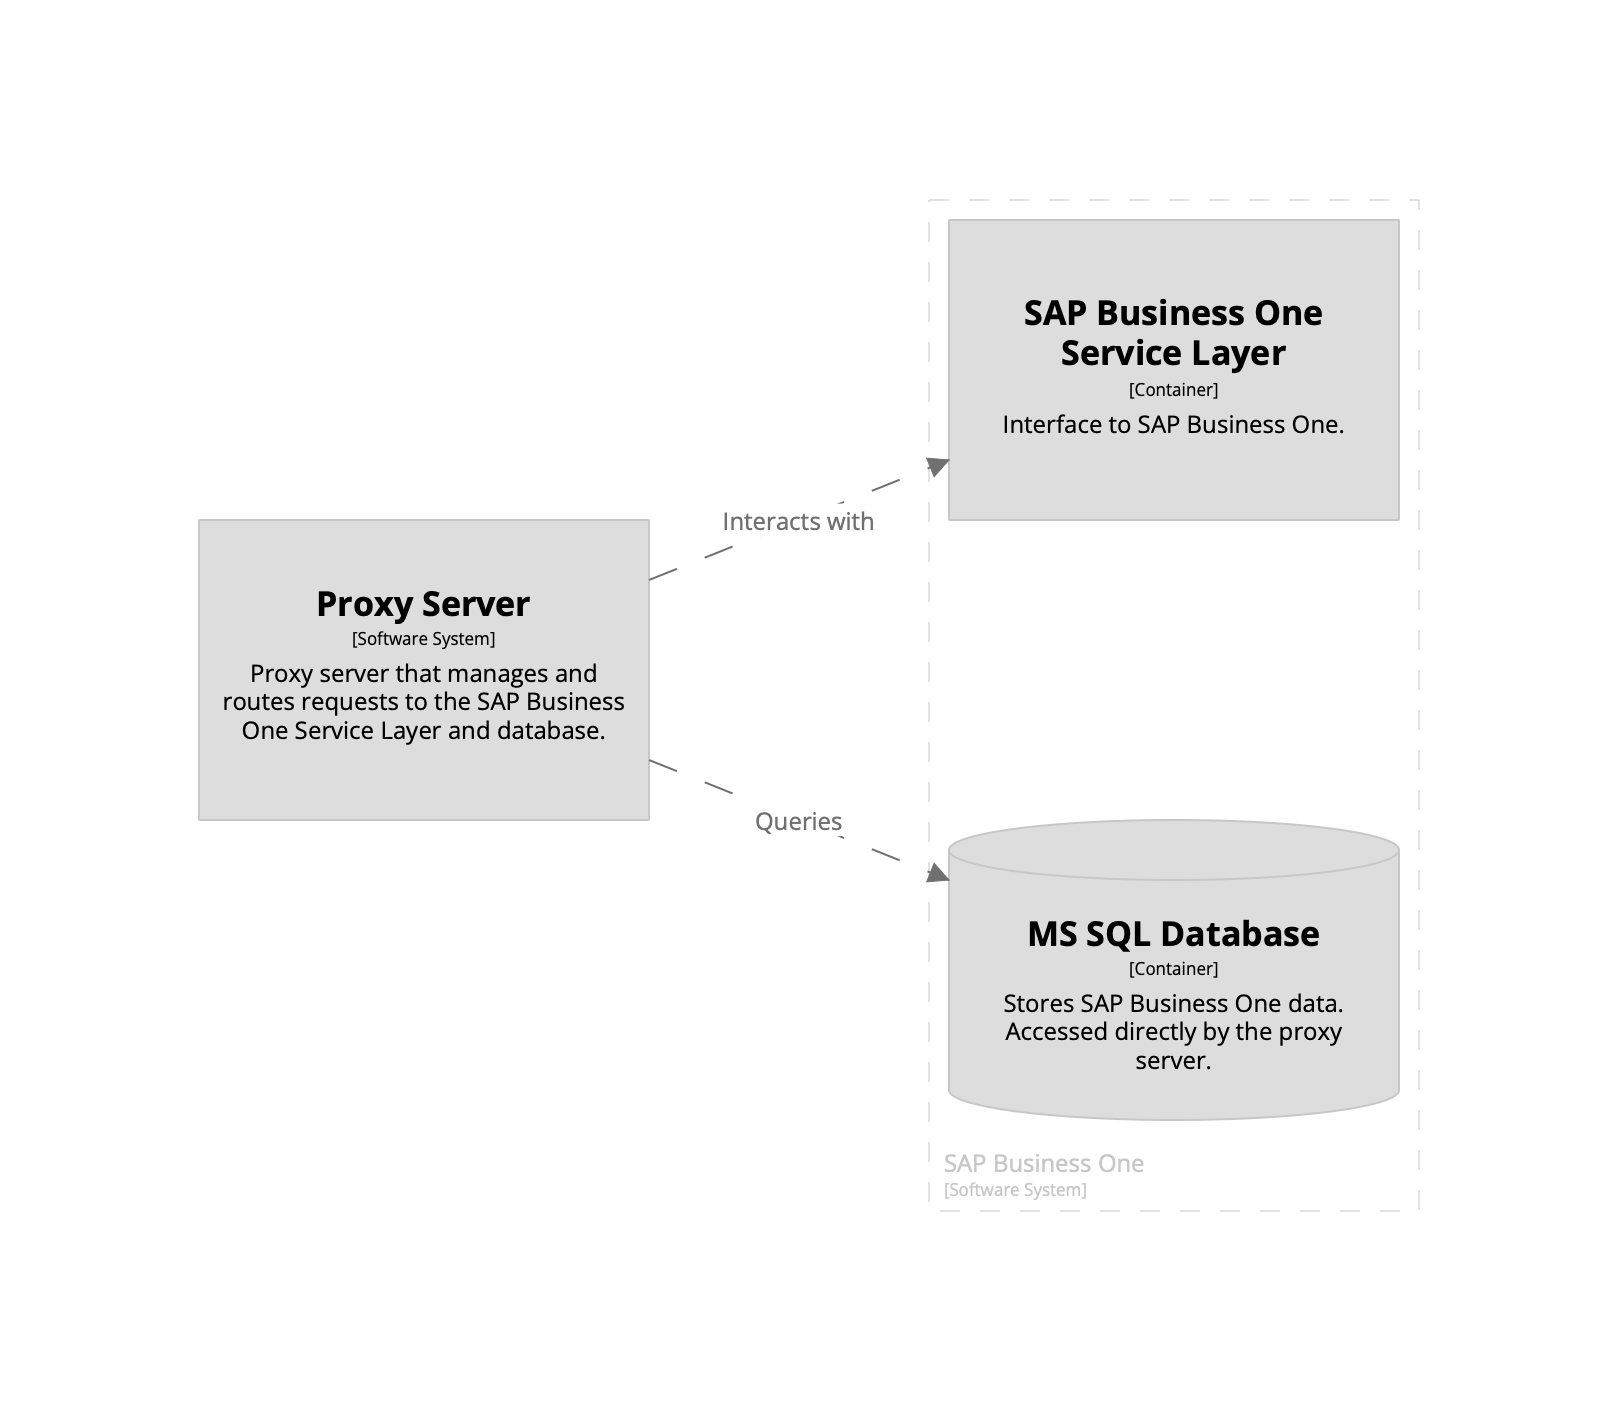
\includegraphics[width=140mm]{img/chap07/fig_structurizr-sap-system.png}
\caption{C4 System diagram of SAP Business One}
\label{img07:structurizr:system:sap}
\end{figure}

A more detailed examination provided in Figure \ref{img07:structurizr:system:proxy} presents the components that make up the Proxy Server, including:

\subsubsection{Reverse proxy as the entry point}
As the entry-point, the front-facing reverse proxy was chosen.
Managing and directing incoming traffic to the Proxy app service

\subsubsection{Proxy app and database}
The proxy application with its own database is the heart of the system.
They are responsible for user management as well as maintaining SAP Service Layer access tokens for both environments and connection pools to both Microsoft SQL database environments.

In contrast to the Proxy system, within our scope, the SAP Business One system is visualised in Figure \ref{img07:structurizr:system:sap} consisting of the following key components (simplified for clarity):
 
\subsubsection{SAP Business One Service Layer}
Running instance of SAP Business One Service Layer installed locally on the server with SAP Business One and the database. 
The Service Layer is accessible via HTTP on a given port.

\subsubsection{SAP Database}
Underlying database used by the SAP Business One instance.
In our case, we are talking about a Microsoft SQL database.


\subsection{Implementation}
\label{subsec:implementation}
% KoaJS app simmilar to the Parcelsync backend
In the landscape of application development, especially when creating an application that serves as an API proxy, developers are presented with large array of options and tools.
To ensure good maintainability, we have opted to remain within the JavaScript ecosystem by leveraging similar technologies used in the \ref{chap:architectural-design}.
This strategic choice not only leads to a more efficient development process, but also enhances existing expertise and resources by building on familiar technologies.

\subsubsection{Technology Stack}

\begin{itemize}
    \item \textbf{Nginx} front-facing reverse proxy managing incomming traffic to the Proxy API.
    \item \textbf{\texttt{Koa.js}} makes up the backbone of the Proxy API as the backend framework. Its lightweight and middleware-orientated design allows for flexible and modular codebase. 
    \item \textbf{PostgreSQL} is employed for storing SAP Service Layer access tokens as well as user credentials.
    \item \textbf{\texttt{Objection}, \texttt{Knex}} are tools configured to provide seamless integration between \texttt{Koa.js} backend and our database. \texttt{Objection} provides a simple to use ORM where \texttt{Knex} serves as a query builder and database migration management tool.
    \item \textbf{\texttt{Yarn}} is chosen as a package manager and script executor.
\end{itemize}


\subsubsection{Proxy API structure}
The Koa.js backend is structured into several entities, middlewares, services, and actions that ensure modular and maintainable code. 
Objection Models used for Object Mapping entities to the Database.
\begin{itemize}
    \item \textbf{\texttt{User}} basic model used for authentication and authorization. Storing username, password, and role (user/admin).
    \item \textbf{\texttt{SAPToken}} persistent singleton instance of a environment bias token having just token, environment, and expiration time.
\end{itemize}
Each middleware is designed to perform specific functions and, if needed, store additional data in the context passed to the next chained middleware or a final action.
\begin{itemize}
    \item \textbf{Authentication middleware}
    \item \textbf{Authorization middleware}
    \item \textbf{SAP Environment middleware}
    \item \textbf{SAP Service Layer Login middleware}
\end{itemize}
Services usually perform \ac{CRUD} operations on a database using a package \texttt{Objection} as \ac{ORM}. They are most often called from actions; however, in some instances, they are called directly from one of our middlewares.
\begin{itemize}
    \item \textbf{SAP service} provides a log-in to generate, store, and retrieve SAP Service Layer authentication tokens for both environments.
    \item \textbf{User service} provides simple CRUD and authentication methods for user objects.
\end{itemize}
At the end of the middleware chain there are actions.
They serve as the main endpoint function.
In our instance, we only need CRUD operations for manipulating and listing user objects, proxy for SAP Service Layer, and \ac{MS} SQL query method making use of pre-initialised singleton database connection pool for both environments.
\subsubsection{Microsoft SQL connector}
In order to allow for efficient SQL queries directly to the database, the Proxy API implements an endpoint that expects a query in the body.
The query is then forwarded to pre-initialised \ac{MS} SQL connection for either development or production database, based on the user's choice. 
The database connection pool is initialised on application start-up in order to minimise cold-starts.
As a connector to the database, the \texttt{mssql} package for Node.js from \texttt{tediousjs} was used. However, as was later found, this package is not able to keep two distinct connection pools when calling the basic \texttt{login} method.
It stored in cache only, although a different one was required. This was an issue since the requirement was to allow for connection to two different databases. 
However, this behaviour can be overcome by creating a \texttt{ConnectionPool} instance directly instead of relying on built-in login functions and caching it outside of the library.
% todo pridat kod??

\subsubsection{SAP Service Layer Proxy}
Then main part of the application is, as the name suggests, the Service Layer proxy itself. 
Using a static \texttt{AxiosInstance} request is passed with all necessary headers to the SAP Service Layer endpoint expecting a stream in the response.
This approach, of course, creates some overhead by calling the API directly. 

A series of performance tests were conducted to quantify the difference in response times. 
The goal was to evaluate efficiency of the Proxy API while handling authentication, authorization and data forwarding while operating remotely. 
As can be seen in figure \ref{img07:response_times}, on average, direct calls to request the full \texttt{BusinessPartner} object from the SAP Business One Service Layer were completed in approximately 0.085 seconds. 
In contrast, calls made through the Proxy API were executed in an average response time of approximately 0,268 seconds.

Although the Proxy API introduces an additional overhead, resulting in longer response times compared to direct Service Layer interactions, the increase is fairly consistent and within acceptable margins, given the added functionalities and remote location with public domain access which introduces considerable network latency.


\begin{figure}[p]\centering
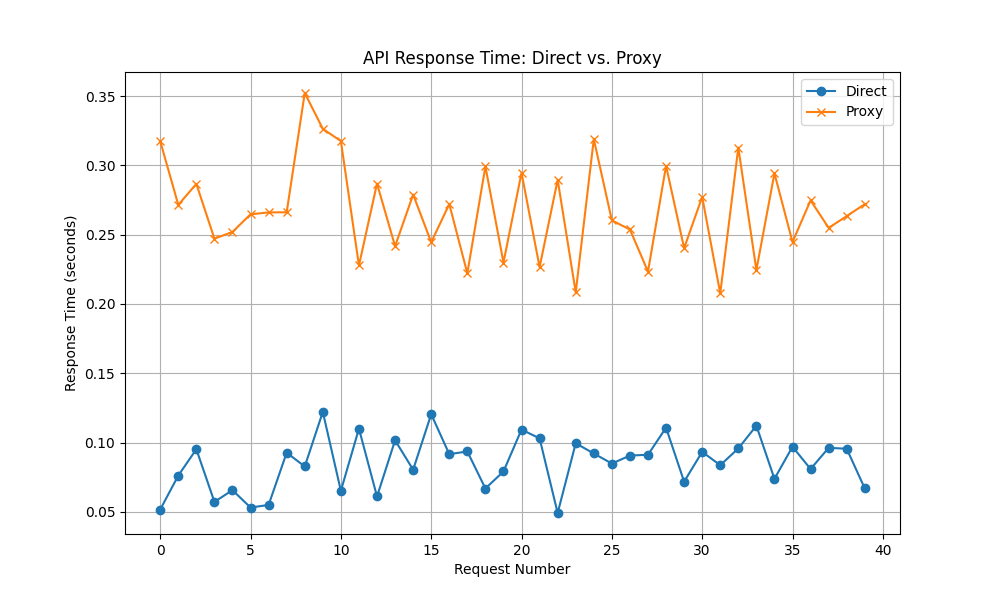
\includegraphics[width=140mm]{img/chap07/fig_api_response_direct_response_time.png}
\caption{Response time of direct SAP Service Layer call in contrast of Proxy API}
\label{img07:response_times}
\end{figure}

\subsubsection{Database model overview}
Database model of the Proxy API is very minimalist and can be best seen in \ref{img07:db_diagram}
Its main focus is to store user data in a safe way. 
In addition, it serves as a cache for SAP Service Layer tokens. 
This approach might initially appear to be an overextension, such as "using a sledgehammer to crack a nut". 
However, our user base might grow, and even for minimal usage of the production instance, it is necessary to provide reliable persistent storage.

\begin{figure}[p]\centering
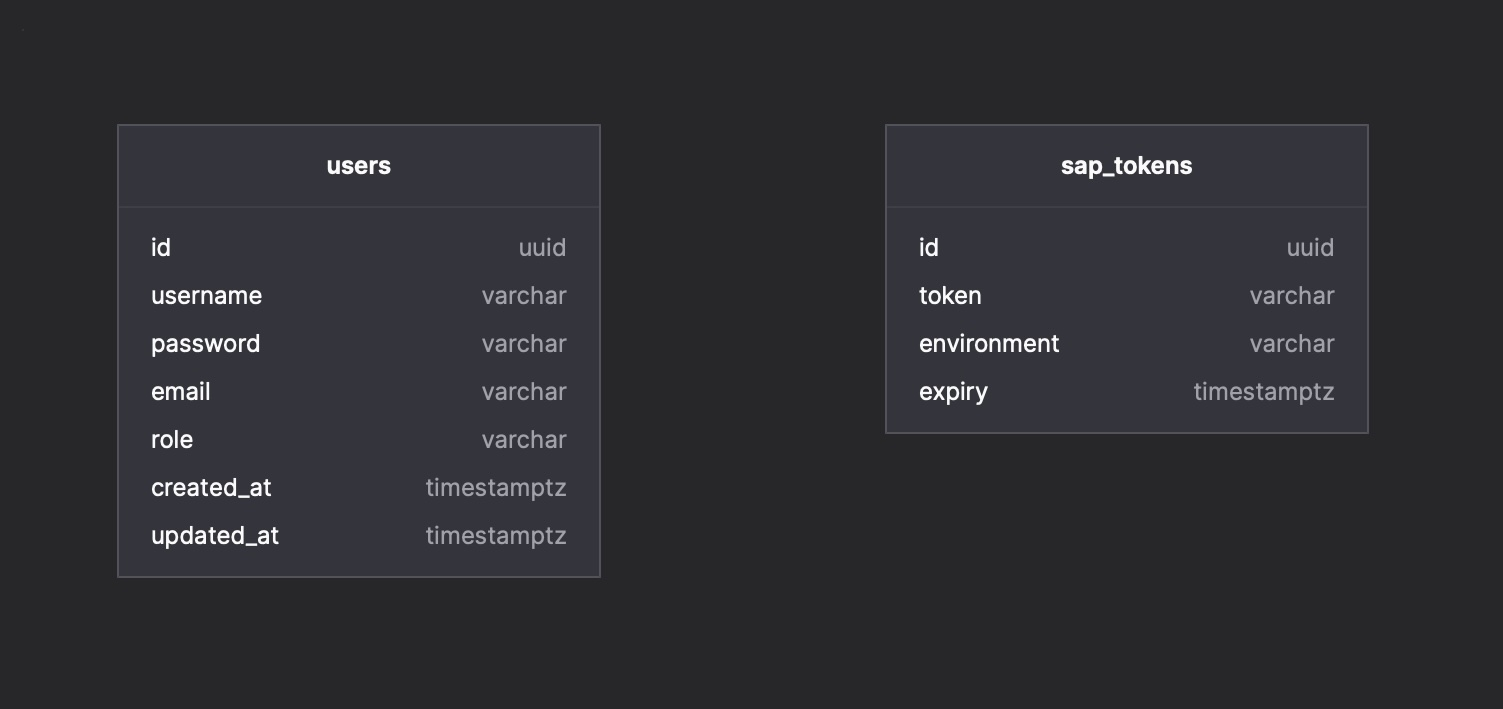
\includegraphics[width=140mm]{img/chap07/fig_db-diagram.jpg}
\caption{DB diagram of database models}
\label{img07:db_diagram}
\end{figure}



\subsection{Deployment}
\label{subsec:deployment}
% Deployed as an containarized application into Docker
% Had to be local to the SAP B1 instance -> Linux VM on the server of company 
The deployment of the Proxy API was carried out on a dedicated Virtual Private Server (VPS) running with Ubuntu 22.04.3 within company's network utilizing modern set of technologies and practices to optimize deployment workflow.

\subsubsection{Overview}
Probably the most significant part of the deployment itself is utilizing Docker, a powerful containerization platform that simplifies the process of building, shipping and running applications in different environments and contexts. 
The container was constructed using a multi-phase Dockerfile, which allows for a seamless streamlined setup by caching dependencies and separating the build process into several phases.
This approach not only speeds up the build process, but it even significantly minimises the footprint of the container itself.


\subsubsubsection{Dockerfile strategy}
The Dockerfile was divided into multiple phases to optimize the build process
\begin{itemize}
    \item \textbf{Dependency Caching:} The initial phase used \texttt{Node.js 18.16.1-bullseye-slim} as the base image to cache package.json file.
    \item \textbf{Build Process:} A temporary image created in the first phase is reused to install dependencies and build the Proxy API using \texttt{esbuild}, JavaScript bundler, and minifier. 
    \item \textbf{Production Image:} The final image was prepared using the same Node.js base image as in the first phase. From this image, all development dependencies and source code were removed to ensure that only necessary components for running the application were included.
\end{itemize}

\subsubsection{Continuous Deployment and Continuous Integration}
\label{subsubsec:cicd}
The build and deployment process was completely automated. 
Automated build is done in an official Docker container registry, a Docker Hub, using GitHub integrations where all source code is stored.
Every push to the master branch triggers a new build on the Docker Hub, ensuring that the latest version of the application was always available.
Deployment on the Linux VPS is managed by \texttt{Watchtower}, an automated update tool that checks for new Docker images every 60 seconds and updates the running container accordingly.
This setup allows for continuous deployment with minimal manual intervention.
Furthermore, Slack notifications were integrated to provide immediate alerts on deployment status and system overall health, allowing quick responses to potential problems.

\subsubsection{Accessing the application}
To securely present the Proxy API to the Internet, Nginx was used as a reverse proxy configured with Certbot for automatic SSL certificate management.
This setup ensures that all traffic to and from the Proxy API is encrypted.
Using this configuration, secure and reliable gateway for accessing the Proxy API was achieved.


\subsection{Data Sender}
\label{subsec:data-sender}
% Write about implementation of a simple Node.JS app which works like an intermidiate between Parcelsync and SAP Proxy

This module serves as an intermediary that covers the data flow between Parcelsync and SAP Business One through the Proxy API, as can be seen in \ref{img07:structurizr:data_sender}
The application written in TypeScript running in a Node.js environment.

\begin{figure}[p]\centering
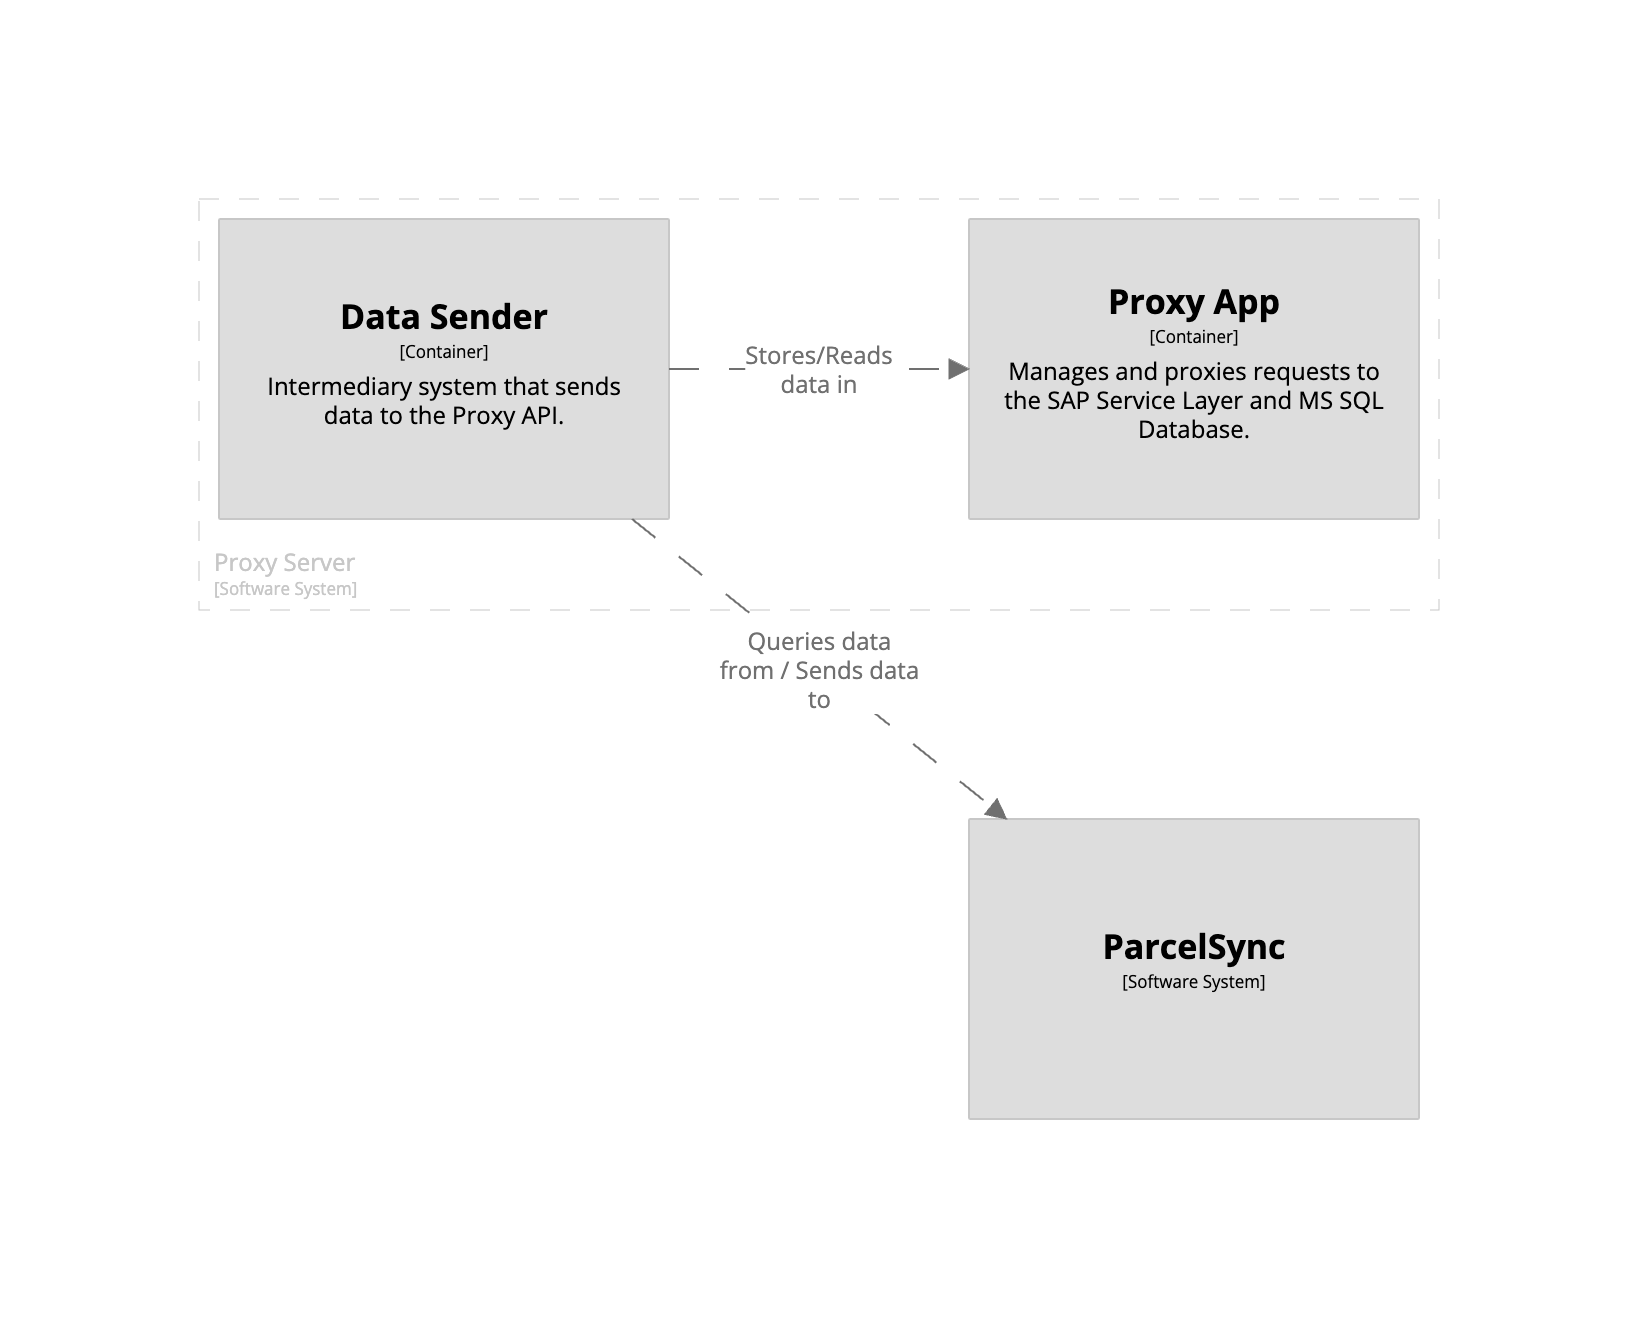
\includegraphics[width=140mm]{img/chap07/fig_data_sender.png}
\caption{C4 Container diagram of communication with SAP}
\label{img07:structurizr:data_sender}
\end{figure}


\subsubsection{Design and Configuration}
The Data Sender module integrates a scheduler that orchestrates task execution based on predefined schedules or commands.
Time-schedule tasks are necessary to ensure that importing new shipments into Parcelsync or updating shipment statuses in SAP are performed efficiently and in expected times.
Using the Node.js package \texttt{node-cron} for scheduling and the \texttt{yargs} library for simple CLI configuration.

\subsubsection{Functionality}
The main entry script acts as the core of the Data Sender.
Initialising the application and setting up scheduled tasks.
Each task is designed to address specific data synchronisation needs between Parcelsync and SAP Business One.
\begin{itemize}
    \item \textbf{Order imports:} Divided by carriers - Packeta, PPL, Ceska Posta, this task targets the retrieval of "unsent" orders reflecting data storage conventions in SAP Business One with option to ship shipment with multiple parcels (tracking numbers).
    \item \textbf{Shipping number imports:} Importing shipping numbers for recently dispatched orders back into SAP, ensuring that the data in SAP Business One stay up to date.
    \item \textbf{Parcel updates:} Focused on updating the information of the parcel in a specific time frame. This task updates shipment status, invoice numbers, and shipping cost in SAP, using Parcelsync status mapping for efficiency.
\end{itemize}

\subsubsection{Deployment strategy}
Similar to the Proxy API \ref{subsec:deployment}, the Data Sender application is containerised, ensuring consistency and reliability across multiple environments.
The CI/CD setup mirrors what was already described in \ref{subsubsec:cicd}, using automated builds and deployments to maintain up-to-date and secure operations. 
The container is designed to be always on utilising the scheduler to continuously check and run tasks.
